\chapter{Nao}
Nao ist ein humanoider Roboter des französischen Herstellers \textit{Aldebaran Robotic}. Die erste Version des Roboters wurde 2006 vorgestellt und unter anderem mit einem Investment durch Intel weiterentwickelt. Es gibt den Roboter in verschiedenen Ausführungen mit verschieden verbauten Sensoren und kostet ungefähr 10.000 Euro. \cite{ws:wikinao}

Im folgenden Kapitel wird der Aufbau und die Funktionen der Hardware, sowie die zugehörige Software zur Bedienung und Programmierung des Nao vorgestellt.

\section{Nao Hardware}
\label{nao:hardware}
Der in dieser Arbeit verwendete Nao ist vom Typ \textit{NAO V3+, V3.2}. Dieser Typ ist 573.2 mm hoch, 290 mm tief und 273.3 mm breit. In Abbildung \myref{f:nao_ov} sind alle Sensoren und Aktoren aufgeführt.
\\
\begin{figure}[H]						
	\centering							
	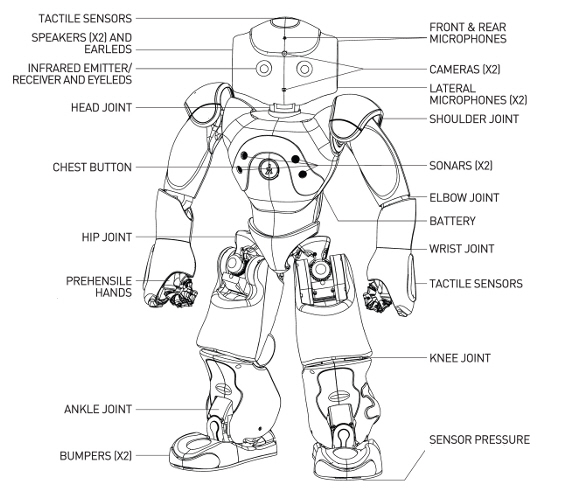
\includegraphics[scale=0.9]{Bilder/nao_overview.jpg}			
	\caption{Übersicht Nao V3.2}						
	\label{f:nao_ov}						
\end{figure}
\noindent
\textbf{Gelenke}
\\
Nao besitzt  im Kopf, den beiden Armen, dem Becken und den beiden Beinen jeweils mehrere Gelenke (\textit{Joint}, siehe Bild \ref{f:nao_ov}). Damit ist eine umfangreiche Bewegung in alle Richtungen der drei Achsen möglich. Der Kopf lässt sich in Z-Richtung drehen und in Y-Richtung neigen, damit Nao auch räumlich sehen bzw. Objekte verfolgen kann.
Die Arme besitzen die gleichen Gelenke wie in einem menschlichen Körper. Dazu gehören Schulter-, Ellenbogen- und Hangelenk. Das Schultergelenk dient dazu, den Arm zu heben/senken und ihn zu öffnen bzw. zu schließen. Das Drehen und Öffnen/Schließen des Unterarms geschieht durch das Ellenbogengelenk in Kombination mit dem Hangelenk. Die Finger der Hand können nur als Ganzes geöffnet bzw. geschlossen werden.
Das Beckengelenk wird dazu benutzt, den Torso von Nao nach vorne oder hinten zu neigen.
Die Beine bestehen aus drei Gelenken: Einem Hüft-, einem Knie- und einem Fußgelenk. Die Bewegungsfreiheit der Beine ähnelt dem des menschlichen Beins, wobei keines der Gelenke in Z-Richtung gedreht werden kann.

Die Bestimmung der Gelenkpositionen erfolgt über einen magnetischen Drehwinkelgeber	mit einer Auflösung von 12 Bit. Das macht beispielsweise bei einem Wert von 4096 pro Umdrehung eine Präzision von 0.1 Grad.
\\
\\
\textbf{Gelenkraum Nao}
\\
Da primär die Arme durch Nao nachgeahmt werden sollen, wird hier kurz auf den Gelenkraum dieser eingegangen. Jedes einzelne Gelenk der beiden Arme besitzt einen Winkelbereich in dem diese bewegt werden können. Tabellen \ref{tab:Lgelenkraum} und \ref{tab:Rgelenkraum} zeigen den Gelenkraum für den linken bzw. den rechten Arm.

\begin{table}[H]
    \begin{tabular}{|l|l|l|}
    \hline
    \textbf{Gelenk}         & \textbf{Bereich (Grad) } & \textbf{Bereich (Radian)}   \\
    \hline
    LShoulderPitch & -119.5 to 119.5 & -2.0857 to 2.0857  \\
    LShoulderRoll  & -18 to 76       & -0.3142 to 1.3265  \\
    LElbowYaw      & -119.5 to 119.5 & -2.0857 to 2.0857  \\
    LElbowRoll     & -88.5 to -2     & -1.5446 to -0.0349 \\
    LWristYaw      & -104.5 to 104.5 & -1.8238 to 1.8238  \\ \hline
    \end{tabular}
    \caption {Gelenkraum linker Arm}
    \label{tab:Lgelenkraum}
\end{table}
\begin{table}[H]
    \begin{tabular}{|l|l|l|}
    \hline
    \textbf{Gelenk}         & \textbf{Bereich (Grad) } & \textbf{Bereich (Radian)}   \\
    \hline
    RShoulderPitch & -119.5 to 119.5 & -2.0857 to 2.0857 \\
    RShoulderRoll  & -76 to 18       & -1.3265 to 0.3142 \\
    RElbowYaw      & -119.5 to 119.5 & -2.0857 to 2.0857 \\
    RElbowRoll     & 2 to 88.5       & 0.0349 to 1.5446  \\
    RWristYaw      & -104.5 to 104.5 & -1.8238 to 1.8238 \\ \hline
    \end{tabular}
    \caption {Gelenkraum rechter Arm}
    \label{tab:Rgelenkraum}
\end{table}
Bilder der einzelnen Gelenke und Winkelbereiche sind im Anhang zu finden.
\noindent
\textbf{Aktoren}
\\
In Nao sind vier verschiedene Typen von Motoren verbaut. Diese unterscheiden sich im wesentlichen in ihrer maximalen Anzahl an Drehungen pro Minute, dem Drehmoment und der Drehzahlrückstellung. Dies ist wichtig, da nicht jedes Gelenk und der zugehörige Aktor mit der gleichen Masse belastet wird.
\\
\\
\textbf{Elektronik \& Sensoren}
\\
Das Herz von Nao ist dessen Motherboard mit einer x86 AMD CPU mit 500MHz. Der Arbeitsspeicher mit 256MB RAM und die 2GB Flash-Speicher befinden sich zusammen mit dem Prozessor im Kopf.  Die Batterie mit rund 30Wh hält für die aktive Nutzung (viele Bewegungen und Sensoraktivitäten) ca. 60min und die normale Nutzung ca. 90min. 

Links und Rechts am Kopf befinden sich jeweils ein Lautsprecher und ein Mikrofon. Zusätliche Mikrofone sind am Kopf auch noch vorne und hinten angebracht. Damit ist es Nao möglich, ein Geräusch zu lokalisiern und gegebenenfalls dahin zu folgen. Um gleichzeitig die Ferne und die Nähe visuell zu verarbeiten wurde über und unter den Augen jeweils eine VGA - Kamera mit einer Auflösung von 640x480 Pixeln installiert. Die Augen selbst dienen zur Erkennung von Infrarotlicht, wobei auch hier in jedem Auge jeweils ein Sensor verbaut ist.

Auf der Brust von Nao befinden sich Ultraschallsensoren zur Distanzermittlung (je 2 Emitter und Empfänger). Diese haben eine Auflösung von 1cm und eine Erkennungsweite von 0.25m bis 2.55m. Unter 0.25m erkennt Nao nur noch, dass ein Objekt im Weg ist, aber nicht wie weit es entfernt ist.

Sensoren zur Kontakterkennung befinden sich auf dem Kopf, dem Brustbutton, auf und neben den Händen, sowie vorne an den Füßen. Unter den Füßen befinden sich zudem noch piezoresistive Drucksensoren mit einem Arbeitsbereich von 0 bis 25 Newton. Damit lässt sich unter anderem erkennen, ob Nao nur auf einem Bein oder auf unebenen Untergrund steht.


\section{Nao Software}
Um Nao auf einfache Weise zu programmieren, simulieren oder ihm neue Funktionen beizubringen, gibt es im wesentlichen zwei Programme. Diese werden im Folgenden jeweils kurz vorgestellt:
\\
\\
\noindent
\textbf{Choregraphe} 
\\
Choregraphe ist eine multi-plattform Desktopanwendung. Mit ihrer Hilfe ist es möglich:
\begin{itemize}
\item Neue Animationen und Verhalten zu erstellen,
\item diese entweder auf einem simulierten  oder direkt auf einem realen Roboter zu testen und
\item den Roboter dabei zu überwachen und zu steuern.
\end{itemize}
Dabei steht die Einfachheit der Anwendung im Vordergrund und so ist es auch möglich, sehr komplexes Verhalten (z.B. Interaktion mit Menschen, Tanzen oder E-Mails verschicken) zu implementieren ohne eine einzige Zeile Quellcode selbst zu schreiben. Zusätzlich ist die Möglichkeit gegeben, vorhandenen Code mit eigenem Python-Code zu erweitern.

\begin{figure}[H]						
	\centering							
	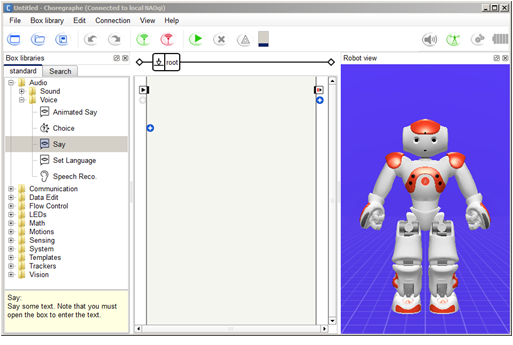
\includegraphics[scale=1.0]{Bilder/choregraphe.png}			
	\caption{Überblick Choregraphe}						
	\label{f:nao_choregraphe}						
\end{figure}
\noindent
Abbildung \ref{f:nao_choregraphe} zeigt einen Überblick über alle Subfenster und Panels innerhalb Choregraphe. Wie zu sehen, ist Choregraphe zentral in drei Bereiche unterteilt: Links, Mitte und Rechts.
Auf der linken Seite ist die sogenannte Box-Bibliothek zu finden. Dort sind alle von Haus aus gespeicherten Bewegungen und Verhalten abrufbar. Diese können per Drag \& Drop in die Mitte gezogen werden. Die Mitte stellt ein Fluss-Diagramm der einzelnen Boxen dar. So ist es möglich \textit{grafisch} zu programmieren (Verknüpfen der Boxen). Auf der rechten Seite ist das Abbild eines Nao-Roboters zu sehen. Dies zeigt, je nach dem, einen simulierten Roboter oder die Spiegelung eines realen Naos. 
Durch diese grafisch einfache Programmierung können auch unerfahrene Anwender mit Nao arbeiten. So ist er nicht nur für die Forschung oder für Entwickler gedacht, sondern auch für den Unterricht an Schulen.

Die Programmierung des Roboters geschieht durch Verbinden von einzelnen Boxen. Es ist auch möglich ein Programm mit verschiedenen Wegen zu entwerfen oder Konditionalstrukturen (\textit{if-else-elseif}) einzubauen. Abbildung \ref{f:nao_choregrapheProg} zeigt ein Programm, in welchem der Roboter zu einer gewissen Position laufen soll. Währenddessen überprüft er mittels Ultraschallsensor, ob ein Hindernis im Weg ist. Bei positivem Ergebnis soll sich der Roboter hinsetzen.

\begin{figure}[H]						
	\centering							
	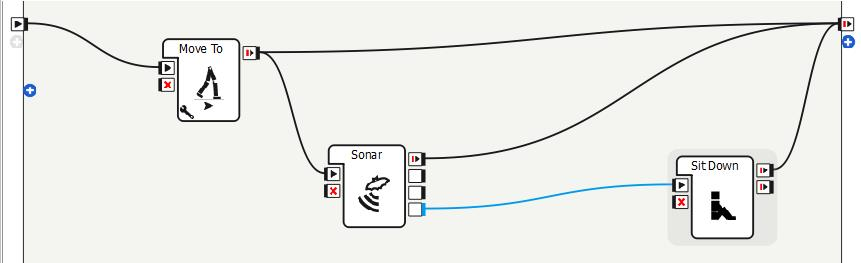
\includegraphics[scale=.6]{Bilder/choregraphe_prog.jpg}			
	\caption{Choregraphe Programmierung}						
	\label{f:nao_choregrapheProg}						
\end{figure}

Neue Bewegungen oder Verhalten können entweder durch eigenen Python-Code oder durch Vormachen integriert werden. Dazu kann über eine \textit{Timeline} aufgenommen werden, zu welchem Zeitpunkt der Bewegung sich die einzelnen Gelenke/Körperteile befinden sollen. Anschließend kann diese aufgenommene Timeline als Verhalten in einer Box gespeichert werden.
\\
\\
Die Möglichkeit neue Programme erst an einer Simulation zu testen, spart erstens Akkulaufzeit eines realen Nao und zweitens schützt es diesen vor \textit{schlechten} Programmen, bei denen er Schaden nehmen könnte. Ein weiterer Vorteil ist, dass zu jeder Box der Quellcode in Python sichtbar ist und sich dadurch Arbeit erspart werden kann.
\\
\\
Choregraphe wurde in dieser Arbeit hauptsächlich dazu genutzt, sich in die Marterie Nao einzuarbeiten, seine Funktionsweise zu verstehen und zu erlernen wie er programmiert wird.
\\
\\
\textbf{Webots for Nao}
\\
Webots für Nao erlaubt es, einen simulierten Roboter in einer virtuellen Welt zu bewegen. Die Software bietet eine sichere Umgebung, um neue Verhalten zu testen, bevor sie in die reale Welt übertragen werden. Webots for Nao ist eine spezifische Auskopplung von Webots 7, einer professionellen Software zum Simulieren diverser Roboter, beispielsweise KUKA-Robotern oder Lego Mindstorms. Mit Webots for Nao können jedoch keine anderen Roboter genutzt oder neue erstellt werden.

\begin{figure}[H]						
	\centering							
	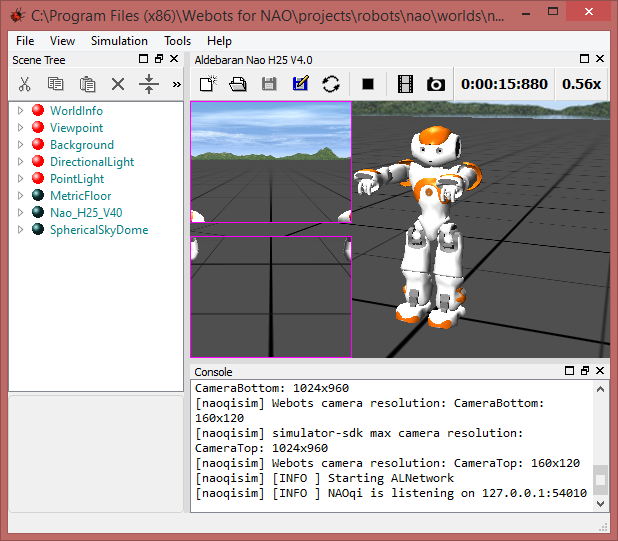
\includegraphics[scale=1.0]{Bilder/webots.png}			
	\caption{Überblick Webots}						
	\label{f:nao_webots}						
\end{figure}
\noindent
Bild \myref{f:nao_webots} zeigt einen simulierten Nao in einer virtuellen Welt. Auf der linken Seite befinden sich Reiter, die ausgeklappt werden können. Dort können Objekte in die Welt gelegt werden. Auf der rechten Seite ist Nao von vorne und jeweils ein Ausschnitt der beiden Kameras an seinem Kopf zu sehen. Unterhalb davon ist eine Konsole, die verschiedene Angaben ausgibt, z.B. die IP-Adresse und der Port, unter dem der simulierte Nao angesprochen werden kann.

Der Unterschied zu der Simulation in Choregraphe liegt darin, dass in Webots auch Elemente wie Tische, Stühle oder andere Hindernisse in die Welt gelegt werden können. So kann beispielsweise getestet werden, ob Nao Hindernissen ausweicht, wenn er auf sie zu läuft.
\\
\\
Webots wurde im Allgemeinen dafür genutzt zu Testen, ob die Übertragung der Armwinkel korrekt ist und ob diese der Bewegung durch den Menschen entsprechen. Würden die Tests an einem realen Nao durchgeführt werden, währen seine Aktoren sehr schnell warm und könnten eventuell Schaden davon nehmen.






\section{NAOqi Framework}

NAOqi ist der Name der Software die tatsächlich auf dem Roboter läuft und ihn kontrolliert. Das NAOqi Framework ist das Gerüst um Nao zu programmieren. Es spricht auf die gewöhnlichen Anforderungen in der Robotertechnik an: Parallelität (von Threads), Ressourcen, Synchronisation und Events. Das bedeutet, es kann mit allen gängigen Techniken der Software - Entwicklung bedient werden. 

Dieses Framework erlaubt homogene Kommunikation zwischen verschiedenen Modulen (Bewegung, Autio, Video), homogene Programmierung und homogenes Teilen von Informationen über die verschiedenen Module hinweg.
\\
\\
\noindent
\myref{f:naoqi_ov} zeigt die einzelnen Komponenten des NAOqi Frameworks:
\begin{itemize}
\item Cross - Plattform
\item Cross - Language
\item NAOqi - Prozess
\item Module
\end{itemize}

\begin{figure}[H]						
	\centering							
	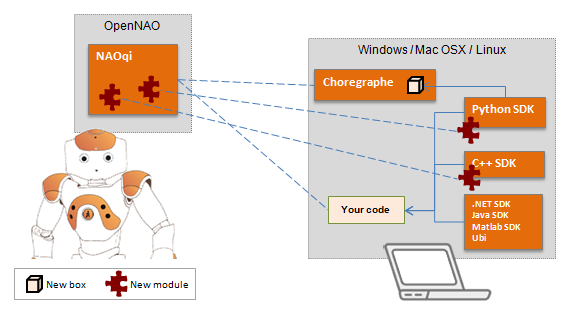
\includegraphics[scale=0.8]{Bilder/naoqi_ov.PNG}
	\caption{NAOqi Übersicht}						
	\label{f:naoqi_ov}						
\end{figure}


\subsection{Cross - Plattform/Language}

\textbf{Cross - Plattform}
\\
Cross - Plattform bedeutet Plattformunabhängigkeit gegenüber dem Betriebssystem auf dem Programmiert werden soll. Sowohl auf Linux, Windows und auf Mac kann Code für Nao programmiert werden. Allerdings kann auf Windows und Mac nur Code auf dem Computer selbst kompiliert werden, während auf Linux der Code auch auf dem Roboter selbst programmiert werden kann.
\\
\\
\textbf{Cross - Language}
\\	
Cross - Language ist nach \cite{ws:naodocu} die Eigenschaft, dass Software in C++ und in Python entwickelt werden kann. In allen Fällen, in denen die Methoden exakt gleich sind kann die \ac{API} (dt: Programmierschnittstelle), gleichgültig von welcher der unterstützten Programmiersprachen, aufgerufen werden. Die \ac{API} ist in acht Programmiersprachen verfügbar: C++, Python, .NET (C\#, Visual Basic, F\#), Java, Matlab und Urbi.

Neue NAOqi Module können nur in C++ oder Python entwickelt werden, jedoch kann die Client - API mit allen Programmiersprachen angesprochen werden. Ebenso sind nur C++ und Python auf dem Roboter unterstützt, die anderen Sprachen werden nur über \textit{Remote - Access} unterstützt. (siehe unten \textit{Proxy})
\\
\subsection{NAOqi - Prozess}
Der NAOqi - Prozess der auf dem Roboter läuft ist ein \textit{Broker} (siehe unten). Beim Start des Prozesses wird eine Konfigurationsdatei \textsf{autoload.ini} geladen, die definiert, welche Bibliotheken geladen werden sollen. Jede Bibliothek beinhaltet ein oder mehrere Module, die der Broker nutzt um deren Methoden öffentlich anzuzeigen. (siehe \ref{f:naoqi_broker1})

\begin{figure}[H]						
	\centering							
	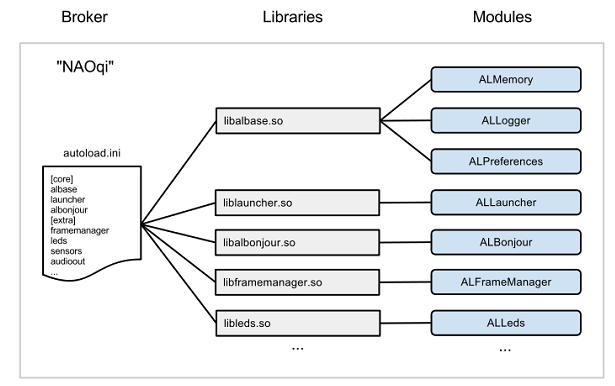
\includegraphics[scale=0.8]{Bilder/naoqi_process1.PNG}
	\caption{NAOqi Broker}						
	\label{f:naoqi_broker1}						
\end{figure}

Der Broker 	stellt einen Lookup - Service zu Verfügung, so dass jedes Modul im Baum oder verteilt im Netzwerk jede Methode finden kann, die öffentlich angezeigt wurde.

Das Laden der Module zum Start erzeugt einen Baum von Methoden, die an Module geknüpft und diese wiederum an einen Broker geknüpft sind. (siehe \ref{f:naoqi_broker2})

\begin{figure}[H]						
	\centering							
	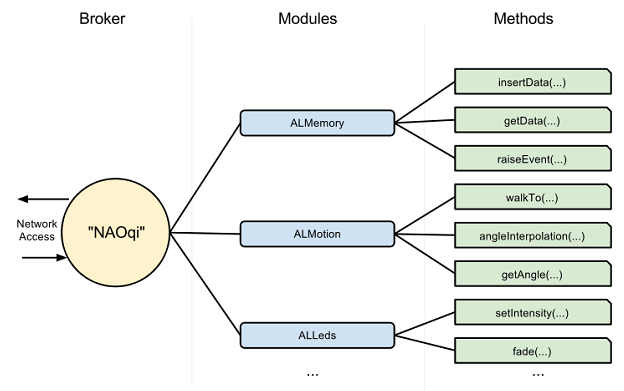
\includegraphics[scale=0.8]{Bilder/naoqi_process2.PNG}
	\caption{NAOqi Method-Tree}						
	\label{f:naoqi_broker2}						
\end{figure}
\noindent
\textbf{Broker}
\\
Der Broker ist ein Objekt, der zwei generelle Rollen einnimmt. Erstens ist das ein Verzeichnis - Dienst, mit dessen Hilfe Module und Methoden gefunden werden können und zweitens ein Netzwerk - Anschluss, der es möglich macht Methoden verknüpfter Module auch außerhalb des Prozesses aufzurufen.

Die Meiste Zeit muss sich keine Gedanken um die Broker gemacht werden, da diese ihre Arbeit selbstständig und transparent machen. Geschriebener Code kann gleich sein, ob für Aufrufe an "`remote Module"' (dt.: entfernt; anderer Prozess oder anderes System) oder "`lokale Module"' (gleicher Prozess).
\\
\\
\textbf{Proxy}
\\
Ein Proxy ist ein Stellvertreter - Objekt das sich genau so verhält, wie das Modul das es repräsentiert. Wenn ein Proxy - Objekt des ALMotion Moduls instanziiert wird, erhält das Proxy - Objekt auch alle Methoden des ALMotion Moduls.

Um ein Proxy eines Moduls zu instanziieren gibt es zwei Möglichkeiten: 
\begin{itemize}
\item Nur den Namen des Moduls benutzen. In diesem Fall muss der auszuführende Code und das Modul das verbunden werden soll im selben Broker liegen. Dies ist ein "`lokaler"' Aufruf
\item Zusätzlich zum Namen des Moduls auch die IP und den Port des Broker benutzen. In diesem Fall muss das Modul im zugehörigen Broker liegen. Dies ist ein "`remote"' Aufruf.
\end{itemize}
Der genaue Unterschied zwischen "`remote"' und "`lokalen"' Modulen wird im folgenden erklärt.
\\
\subsection{Module}
Typischerweise ist ein Modul eine Klasse innerhalb einer Bibliothek und wird automatisch instanziiert wenn diese  durch \textsf{autoload.ini} geladen wird. Neue Methoden können an Klassen gebunden werden, die von \textsf{ALModule} erben. Dadurch werden die Methoden mit ihrem Namen und ihrer Signatur dem Broker öffentlich gemacht, so dass diese anderen verfügbar wird.

Ein Modul kann, wie oben bereits erwähnt, entweder "`remote"' oder "`lokal"' sein. 

\textbf{Lokale Module } sind zwei (oder mehr) Module, die im selben Prozess gestartet wurden. Sie kommunizieren miteinander lediglich über \textbf{einen} Broker. Durch den gemeinsamen Prozess können sie sich  Variablen teilen und einander Methoden ohne Serialisierung oder Netzwerkverbindung aufrufen. Dies erlaubt die schnellste Kommunikation untereinander. Lokale Module werden als Bibliothek kompiliert und können ausschließlich auf dem Roboter ausgeführt werden. Sie sind sehr schnell und effizient im Umgang mit dem Arbeitsspeicher.

\textbf{Remote Module} kommunizieren über das Netzwerk miteinander. Jedes remote Module benötigt einen Broker um mit anderen Modulen zu sprechen. Der Broker nutzt dabei das Netzwerkprotokoll SOAP\footnote{Simple Object Access Protocol, dient u.a. dazu \textit{Remoe Procedure Calls} durchzuführen} um die Kommunikation bereitzustellen. Schnelles Ansprechen von Modulen ist über ein remote Modul nicht möglich, beispielsweise bei direkter Adressierung des Arbeitsspeichers. Remote Module werden als ausführbare Dateien kompiliert und können außerhalb des Roboters aufgerufen werden. Remote Module sind einfacher zu benutzen und können dadurch von außen einfacher debuggt werden. Allerdings sind sie langsamer und weit weniger effizient wie lokale Module. 
\\
Die Kommunikation zwischen remote Modulen kann über zwei Wege erfolgen. Erstens \textbf{Broker to Broker} und zweitens \textbf{Proxy to Broker}.
 
Der Unterschied liegt darin, dass Broker to Broker eine wechselseitige, Proxy to Broker nur eine einseitige Kommunikation eröffnet. Bei zwei Modulen B und C kann bei Broker to Broker B Methoden von C und C Methoden von B aufrufen. Bei Proxy to Broker ist dies nur in die Richtung von B nach C möglich, nicht umgekehrt. Folgendes Listing zeigt die Implementierung beider Kommunikationsarten.

\lstinputlisting
    [caption={Kommunikationsarten Module}
       \label{test},
       captionpos=b]	
 {Listings/module_comm.cs}
\noindent	
\textbf{Blocking und non - Blocking Aufrufe}
\\



\subsection{.NET SDK}
vorstellung c\# SDK, HelloWorld
